\section*{Résumé}
\textit{Les cellules solaires photovoltaïques sont généralement modélisées avec un circuit électrique comprenant un certain nombre de composants localisés. Les paramètres de ces composants déterminent la précision de ces modèles mais ne sont généralement pas fournis par les fabricants. Cependant il est possible d'estimer ces paramètres avec la caractéristique I-V de la cellule ou du module PV en se basant sur des techniques numériques ou analytiques. Les méthodes évolutionnaires tel que l'évolution différentielle prennent le problème d'un point de vue d'optimisation mathématique dont la fonction objectif à minimiser étant l'erreur entre la caractéristique calculée du modèle et les données expérimentales. Dans ce travail nous analysons la performance de l'évolution différentielle appliquée aux modèles simple et double diode avec la fonction W de Lambert. De plus, on propose une stratégie métaheuristique pour déterminer les paramètres de l'évolution différentielle pour optimiser le temps de convergence.
}
\section*{Abstract}
\textit{Solar PV cells are generally represented by a lumped-element model with a set number of components which are represented by their parameters. These parameters are not readily available in manufacturer data-sheets despite being crucial to the accuracy of the model. A possible approach is to estimate these parameters using the Current-Voltage characteristic of a cell using numerical or analytic techniques. Metaheuristics such as Differential Evolution take the approach of an optimization problem with the objective function to be minimized being the error with experimental Current-Voltage data. This work is an analysis of the performance of Differential Evolution applied to the single and double diode models with the Lambert W function on various solar cell technologies. A further metaheuristic strategy to determine the parameters of differential evolution is proposed using a higher-order differential evolution in order to speed convergence. A tool implementing these methods has been developed using the Python programming language.}


\printnomenclature

%\section*{Nomenclature}
%\noindent\textbf{GHG} \hfill Green House Gas \hfill Gaz à effet de serre\\
%\textbf{DE} \hfill Differential Evolution \hfill \phantom{}\\
%\textbf{$E_g$} \hfill Bandgap\\
%\textbf{EQE} \hfill External Quantum Efficiency

\newpage
\tableofcontents
\newpage

\chapter*{Introduction Générale}
\label{sec:intro}
\addcontentsline{toc}{chapter}{\nameref{sec:intro}}
%inexhaustible en principe
L’épuisement des énergies fossiles et leur nature non-durable a conduit à la croissance rapide des énergies renouvelables comme sources alternatives d'énergie. L’énergie solaire est l’une de ces sources renouvelables les plus répandues et a prouvé son utilité dans plusieurs domaines d'application grâce à sa nature quasiment inexhaustible. Les technologies photovoltaïques en particulier ont fait l'objet intense d'étude de la part de la communauté scientifique depuis la première cellule en silicium cristallin à 6 \% de Chapin et al. \cite{Chapin1954} en 1954. Ceci a entraîné une croissance considérable de l'industrie photovoltaïque. En fait, la capacité de production en PV a dépassé les 150 GW \cite{iea2020} en 2019 (figure \ref{fig:ieapv}), ce qui correspond une croissance d'environ 100 GW depuis 2014. Les décennies de recherche depuis la cellule de Chapin et al. visent généralement l'amélioration des cellules solaires sur trois axes: \textit{(i)} en explorant les différentes architectures possibles des cellules, \textit{(ii)} en développant des matériaux qui permettent d'augmenter l'efficacité de conversion de l'énergie solaire incidente ou \textit{(iii)} en réduisant le coût du processus de production. La première génération des technologies PV se basait sur des wafers de silicium comme matériau actif de conversion. La deuxième génération remplace le silicium avec des semi-conducteurs à couches minces, qui, parmi d'autres avantages, réduisent considérablement les besoins en matières premières. Les troisièmes et futures générations comprennent les cellules organiques, Perovskite et les Quantums Dots etc. et présentent des pistes d'investigations pour réduire davantage les coûts de production et augmenter l'efficacité de conversion.

Le principe de fonctionnement des cellules photovoltaïques a été discuté en profondeur dans la littérature \cite{Fraas2010,  Sze2006, Wenham2013}.
Les photons à énergie supérieure au bandgap du matériau semi-conducteur sont absorbés en transférant leur énergie aux électrons dans la bande de valence, ce qui leur permet de passer vers la bande de conduction en laissant un "trou" derrière. Le rôle du champ électrique présent dans la zone de déplétion des jonctions P-N est de séparer ces paires électron-trou et leur permettre de circuler à travers une charge extérieure. Toutefois, il y aurait toujours un plafond sur ce mécanisme de conversion "lumière $\rightarrow$ électricité" pour les cellules mono-jonction selon la limite Schockley-Queisser (SQ) \nomenclature{SQ}{Formalisme Shockely-Queisser} \cite{Shockley1961}. Le modèle SQ postule que tous les photons à énergie supérieure au gap $E_g$ sont absorbés et que la totalité des recombinaisons qui surviennent sont strictement l'inverse du processus d'absorption, c'est-à-dire des recombinaisons radiatives qui réémettent des photons.\\
Cependant, la performance d'une cellule réelle sera toujours inférieure à la limite SQ (figure \ref{fig:natsq}). Les mécanismes idéaux postulés par le formalisme de SQ sont affectés dans la pratique par plusieurs phénomènes imprévus qui parviennent des propriétés des matériaux utilisés. À titre d'exemple, la présence des défauts dans un semi-conducteur entraîne des recombinaisons non-radiatives où l'énergie des électrons est libérée en phonons dans la structure cristalline et non pas en photon, ainsi que la recombinaison Auger où un autre électron reçoit cette énergie. Les difficultés qui limitent les technologies PV nécessitent une meilleure compréhension des phénomènes physiques complexes impliqués, et l'étude de la performance des cellules par rapport au modèle SQ donne des indices sur la nature des gains en performance qu'une technologie particulière a le potentiel de réaliser.

La modélisation des cellules solaires s'avère nécessaire par conséquent. Elle est essentielle pour la conception, l'analyse et l'estimation de la performance des cellules solaires. Elle permet d'effectuer l'analyse des propriétés électriques pendant leur phase de développement, l'émulation des systèmes PV pour la prédiction des rendements énergétiques \cite{Ram2018}, le contrôle de qualité des cellules en phase de production %\cite{} 
et l'étude des effets de dégradation pendant la phase d'opération \cite{Kennerud1969, Jamil2017}. Bien qu'il y ait des méthodes de simulation des phénomènes physiques dans la cellule comme celles qui reposent sur la dynamique moléculaire, la théorie fonctionnelle de la densité ou tout simplement des méthodes numériques appliquées aux équations des semi-conducteurs (équation de Poisson et équations de continuité), etc. Dans ce travail nous nous intéressons à l'approche des circuits équivalents à éléments localisés qui modélisent le comportement I-V de la cellule.

La modélisation d'éléments localisés permet de décrire le comportement des systèmes physiques dispersés spatialement avec un ensemble d'éléments localisés dont chacun représente un phénomène physique particulier. L'analogie électrique dans les problèmes de transferts de chaleur est un exemple de cette méthode où une résistance localisée dans le modèle pourrait représenter la résistance thermique spatialement distribuée selon l'épaisseur de la paroi concernée. Dans le cas des cellules PV, chaque élément du circuit équivalent représente aussi un phénomène physique spécifique dans la cellule (e.g. une résistance en série modélise les pertes ohmiques causées par la résistance intrinsèque au semi-conducteur utilisé). Puisque la caractéristique I-V dépend entièrement des paramètres associés aux éléments localisés du circuit. Il s'agirait donc d'essayer de minimiser l'erreur entre la courbe caractéristique du modèle et celle de la cellule réelle en jouant sur les valeurs des paramètres. 
Pour ce faire, il existe deux approches principales. La première est l'approche analytique. Elle consiste à utiliser les données sur les points clés de la courbe caractéristique (tension circuit ouvert, courant court-circuit, la pente de la courbe en ces points, ou encore le point de puissance maximale etc) et à effectuer certaines simplifications pour concevoir des formules approximatives, mais rapide à calculer. Toutefois, les simplifications effectuées peuvent conduire à des résultats imprécis ou non physiques (e.g. résistance négative). De plus, le fait que cette approche utilise les données des quelques points seulement la rend vulnérable aux bruits de mesures. La deuxième approche est l'extraction numérique. On se retrouve avec un problème d'optimisation, dont la fonction objectif à extrémiser (minimiser) est l'erreur entre le modèle et la courbe expérimentale de la cellule réelle. L'algorithme utilisé pour l'optimisation en soi pourrait être déterministe comme dans le cas des méthodes de Newton-Raphson, Levenberg–Marquardt etc. ou des algorithmes stochastiques/métaheuristique comme les techniques évolutionnaires. Ces dernières comprennent l'algorithme génétique (GA) \nomenclature{GA}{Algorithme Génétique}, l'Optimisation par Essaims Particulaires (PSO)\nomenclature{PSO}{Optimisation par Essaims Particulaires (\textit{Particle Swarm Optimization})}, Recuit Simulé (SA) \nomenclature{SA}{Recuit Simulé (\textit{Simulated Annealing})} etc. Les méthodes déterministes imposent généralement des critères de convexité, différentiabilité (et par conséquent continuité) de la fonction objectif. Bien qu'elles soient efficaces en termes d'optimisation locale avec l'accès aux6 données de gradient, elles sont très susceptibles à se piéger dans des extremums locaux, ce qui limite leurs capacités d'optimisation globale. Par contre les métaheuristiques n'ont pas d'exigences sur la fonction objectif, et le choix des conditions initiales appropriées les rend plus robustes envers les pièges d'extremums locaux.

Dans ce travail, après avoir discuté le concept de modélisation par circuits électriques des cellules PV, nous présenterons la technique de l'évolution différentielle proposée par Storn et Price en 1995 \cite{Storn1995}. Comme les autres techniques évolutionnaires, elle consiste à générer une population de solutions sur laquelle on effectue des opérations de mutation et de croisement pour sélectionner les solutions qui constitueront la génération suivante. Ensuite nous allons synthétiser l'ED avec la modélisation par circuits électriques en utilisant la fonction W de Lambert. Nous analysons la performance de l'ED en la comparant avec les autres techniques disponibles dans la littérature avant de conclure en proposant une stratégie pour mieux sélectionner les paramètres de l'ED et optimiser la convergence et le temps de calcul.
\begin{figure}
  \begin{center}
    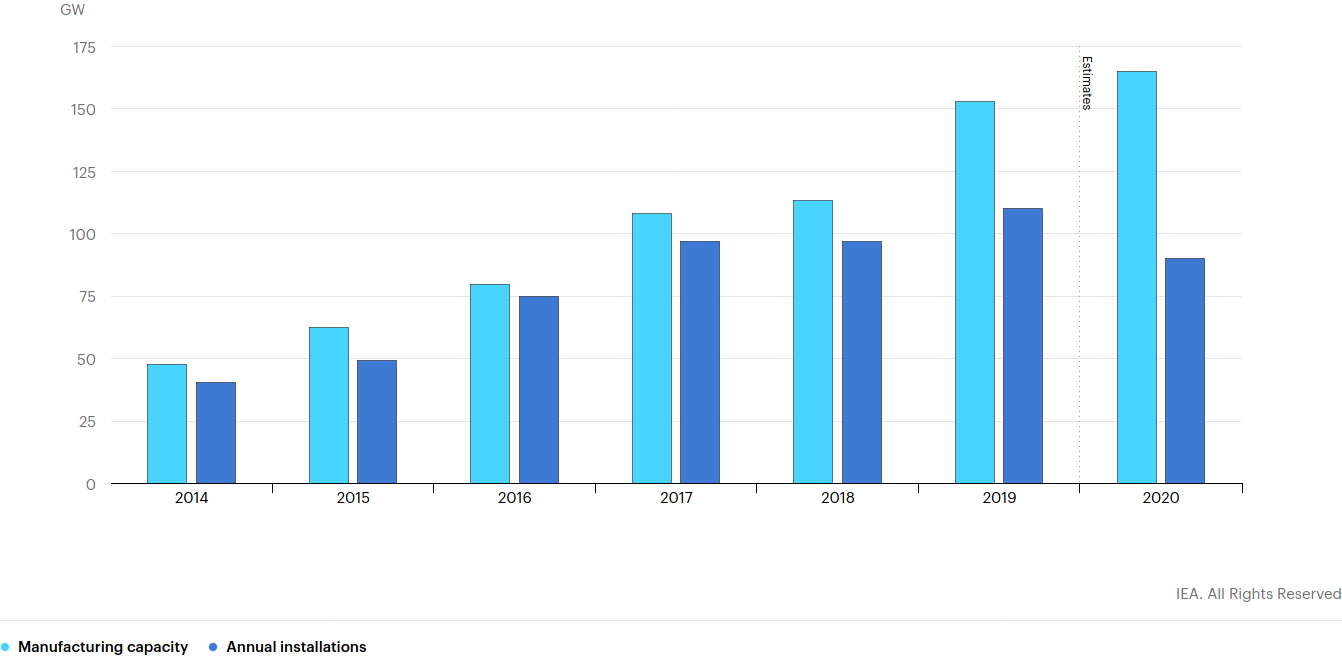
\includegraphics[width=\textwidth]{resources/ieapv.png}
    \caption{Fabrication et demande des modules solaires photovoltaïques, 2014-2020. Source: IEA analysis based on Paula Mints (2020), The Solar Flare, SVP Market Research, San Francisco, CA \cite{iea2020}}
    \label{fig:ieapv}
  \end{center}
\end{figure}
\begin{figure}
  \begin{center}
    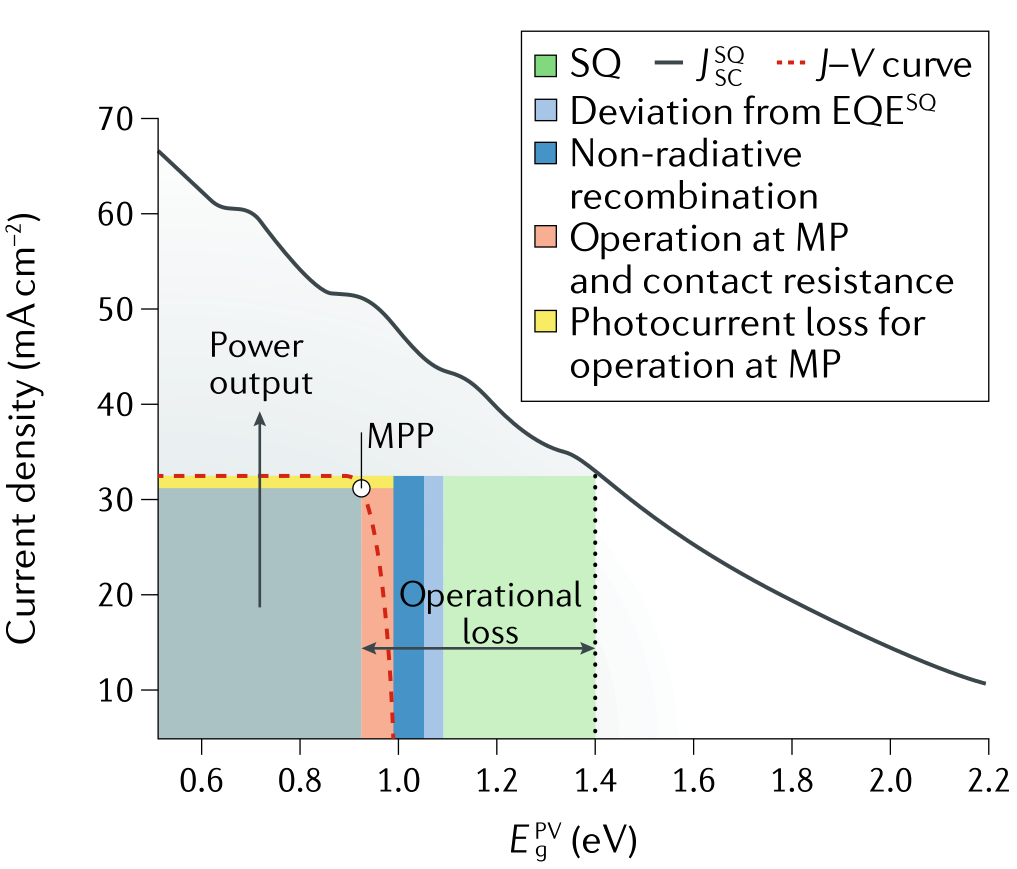
\includegraphics[width=0.8\textwidth]{resources/natsq.png}
    \caption{Différence entre le formalisme de SQ et une cellule réelle. Le photo-courant maximal CC à la limite de Schockley-Queisser est tracé en fonction du gap ($E_{g}^{PV}$). La ligne pointillée en rouge indique la caractéristique J-V de la cellule \cite{nayak2019}}
    \label{fig:natsq}
  \end{center}
\end{figure}
